\chapter{Troubleshooting This Template}\label{appx:troubleshoot}
In this chapter, we detail solutions to common issues that we have encountered when using this template, particularly issues that one may encounter when pasting work that one has already written into it.
While this list is certainly not exhaustive, we hope it may be of some use if your document fails to compile or does not look as you expect.

\section{Conflicting or Incompatible Packages}
As mentioned in \autoref{ch:usage}, there are a number of packages which are currently not compatible with PDF tagging; a \href{https://latex3.github.io/tagging-project/tagging-status/}{list of compatible and incompatible packages} is available from the \LaTeX\ Tagged PDF Project.
We \textit{strongly recommend} starting your thesis with a minimal preamble---modeled after the example provided by this template---and judiciously adding new packages only as you need them.
Almost anything you can hope to achieve in your thesis can be done without using one of these conflicting packages.

\section{Backwards Compatibility with \texttt{unicode-math}}
Here we mention some common backwards-compatibility issues that you might encounter when pasting legacy \LaTeX\ code (especially using \texttt{amsmath}) into this template, which requires using \href{https://ctan.org/pkg/unicode-math}{unicode-math}.

\subsection{Applying Fonts to Special Characters}
Consider the following example, where we use \texttt{amsmath} with \texttt{unicode-math}:
\begin{verbatim}
  Using \verb|\mathbf{}|     : \( \mathbf{\Phi} \)
  Using \verb|\boldsymbol{}| : \( \boldsymbol{\Phi} \)
  Using \verb|\symbf{}|      : \( \symbf{\Phi} \)
\end{verbatim}
If you compile this example, your compiler will give you the keen warning: \textit{Missing character: There is no ... (U+1D6F7) in font [lmroman10-bold]}, but it will compile nonetheless to give you an output resembling \autoref{fig:mathbf}.
When using \texttt{unicode-math}, you cannot apply bold to Greek characters using the (legacy) \verb|\mathbf| command, which is what the compiler was trying to warn you about.

\begin{figure}[ht]
  \centering
  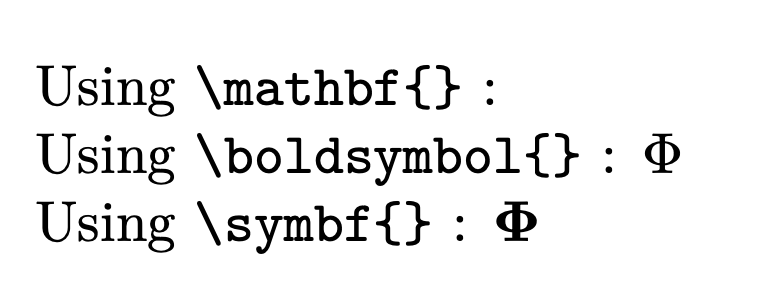
\includegraphics [
    height=3cm,
    alt={The compiled PDF shows nothing for the mathbf code, an essentially normal phi for the boldsymbol code, and a truly bold phi for the symbf code. }
  ]{figs/mathbf.png}
  \caption{Common bug when applying bold to special symbols.}
  \label{fig:mathbf}
\end{figure}

\noindent
This bug is very easy to spot if you are typing a new section of your dissertation from scratch.
Nonetheless, if you are refactoring your existing \LaTeX\ code to use this template, \textsc{beware} that it may compile to give you a PDF but not in the way you intended!
To fix this, you should use \verb|\symbf| instead of \verb|\mathbf|.
Equivalently, you may (carefully) edit the \texttt{tamuthesis.cls} file to load \texttt{unicode-math} with the \texttt{mathbf=sym} option; doing this, you will not have to change anything in your code.
See also this \href{https://tex.stackexchange.com/questions/477680/how-can-i-get-greek-bold-letters}{Stack Exchange post}.

\subsection{Faulty Syntax and Missing Braces}
Without loading \texttt{unicode-math}, some expressions similar to \verb|X^\mathbb{R}| will serendipitously compile and even look `correct' on the page, despite the fact that this is incorrect syntax and \textit{ought} not to compile.
Indeed, it is missing braces: \verb|X^{\mathbb{R}}| would be the correct syntax; see also this \href{https://tex.stackexchange.com/questions/434600/tex-live-2018-unicode-math-does-not-allow-using-mathcal-or-mathbf-as-subscrip}{Stack Exchange post}.
The only real way to fix this is to use the correct syntax.

\subsection{Redefining Common Symbols}
Suppose you want to redefine \verb|\div| so that it typesets the divergence operator (`\( \nabla \cdot \)' or `\( \text{div} \)') instead of the division symbol `\( \div \)'.
One might think to use:
\begin{verbatim}
  \let\div\relax
  \DeclareMathOperator{\div}{\nabla \cdot}
\end{verbatim}
in their preamble.
This will not work as expected in this template, since \texttt{unicode-math} will redefine \verb|\div| one more time as soon as your document begins.
To ensure that your redefinition is loaded \textit{after} that of \texttt{unicode-math}, you should delay it with \verb|\AddToHook{begindocument}| (or the older \verb|\AtBeginDocument|).
For example, adding:
\begin{verbatim}
  \AddToHook{begindocument}{
    \let\div\relax
    \DeclareMathOperator{\div}{\nabla \cdot}
  }
\end{verbatim}
to your preamble will produce the desired behavior.
